
\documentclass[11pt, a4paper, english]{article}
\usepackage{subfigure}
\usepackage{amsfonts}
\usepackage{times}
\usepackage[usenames,dvipsnames]{color}
\usepackage{color}
\usepackage{graphicx}
\usepackage[top=1in,right=1in,left=1in,bottom=1.5in]{geometry}
\usepackage{wrapfig}
\usepackage{amsmath}
\usepackage{authblk}
\usepackage{mdwlist}
\usepackage{listings}
\lstset{
    language=Python,
    backgroundcolor=\color{Dandelion}}
%\usepackage[font=small,labelfont=bf]{caption}
\newcommand{\RR}{\mathbb{R}}
\newcommand{\argmin}{\arg\min}
\newcommand{\half}{\frac{1}{2}}
\newcommand{\comment}[1]{\textit{\color{blue} {#1}}}
\newcommand{\commentout}[1]{}
\newcommand{\deriv}[2]{\frac{\partial {#1}}{\partial {#2}}}
%\newcommand{\vect}[1]{\vec{#1}}
\newcommand{\vect}[1]{\mathbf{#1}}
\newcommand{\xx}{\mathbf{x}}
\newcommand{\x}{\xx}
%\newcommand{\dx}{\mathbf{\delta x}}
\newcommand{\dx}{\mathbf{dx}}
\newcommand{\vv}{\mathbf{v}}
\newcommand{\needref}{$^\textit{reference needed}$}
\newcommand{\tab}{\hspace{5mm}}
\newcommand{\N}[2]{\mathcal{N}\left(#1, #2\right)}
\newcommand{\vmu}[1]{\vect{\mu}_{#1}}
\newcommand{\Nms}[1]{\mathcal{N}\left(\mu_{#1}, \sigma_{#1}\right)}
\newcommand{\NMS}[1]{\mathcal{N}\left(\vmu{#1}, \vect{\Sigma_{#1}}\right)}
\newcommand{\normal}[2]{\frac{1}{\sqrt{2\pi} #2}e^{- \frac{\left(x - #1\right)^{2}}{2 #2^{2}}}}
\newcommand{\Normal}[2]{|2\pi#2|^{-\half} e^{\left(X-#1\right)^T #2^{-1} \left(X-#1\right)} }
\newcommand{\code}[1]{\texttt{#1}}

\title{Symbolic Statistics with SymPy}
\author{Matthew Rocklin}

\date{}
%\includeonly{uqadjoint}
\begin{document}
\maketitle

\section{Introduction}

{\bf blab about symbolics}
We note three increasing trends of scientific computing
\begin{enumerate*}
\item Problems are becoming more complex
\item Computational infrastructure is requiring more attention to detail
\item The average programmer is coming from a less technical background
\end{enumerate*}

That is we need to solve more complex science problems on tricker architectures given less specialized users. To solve this issue we look towards adding additional layers of abstraction in the process of describing problems. For example we no longer ask users to write high performance matrix code, instead we use LAPACK. A layer of abstraction a bit higher in the process is the use of symbolic mathematics.

Commercial software such as Mathematica and Maple exist to aid in these problems. Unfortunately due to their closed nature it is difficult to integrate them into existing code bases. 

{\bf Blab about statistics}
Society is starting to care about uncertainty. 

We introduce random variable types into SymPy allowing high level and intuitive expression of statistical problems. We show how these expressions may then be compiled to a lower-level representation and computed to obtain results in laboratory problems. 

% Motivating Example Section
\section{Motivating Example}
\label{sec:optics}

\begin{wrapfigure}{r}{.4\textwidth}
\vspace{-20pt}
\centering
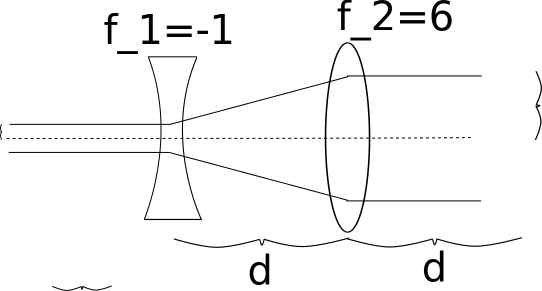
\includegraphics[width=.5\textwidth]{images/beam_expander}
\vspace{-0pt}
\caption{A simple beam expander}
\label{fig:beam_expander}
\vspace{-10pt}
\end{wrapfigure}

To motivate the use of random expressions we build a simple example. Consider the beam expander depicted in figure \ref{fig:beam_expander}. It consists of a thin concave lens of focal length $f_1$, followed by $d$ units of free space, followed by a convex lens of focal length $f_2$, followed by $d$ more units of free space followed by a target. If $f_2 = d-f_1$ then incoming parallel horizontal rays produce outgoing parallel rays. I.e. beams remain beams though their widths may
expand or contract.

If we allow only rays with small angles then such systems can be concisely described using matrices. We build such a system in using the built-in SymPy Gaussian optics module. 

\begin{lstlisting} 
f1 = Symbol('f1')
f2 = Symbol('f2')
d = Symbol('d')

lens1 = optics.ThinLens(f1)
lens2 = optics.ThinLens(f2)
space = optics.FreeSpace(d)

beam_expander = space*lens2*space*lens1

height = 5
angle = 0
ray = optics.GeometricRay(height, angle)

exit_ray = beam_expander * ray
exit_height, exit_angle = exit_ray

\end{lstlisting} 

If we substitute in values $f_1 = -1 , d=5 , f_2=6$ we find that the exit height equals 30, magnified six times, while the exit angle remains 0. 

We now consider a more realistic setting where the device to set the ray's angle has some normally distributed error. In this example we describe te ray's angle with mean zero and standard deviation $pi/100$.

\begin{lstlisting}
angle = Normal(0, pi/100)
\end{lstlisting}

\code{angle} is an object of the RandomSymbol type. It acts like as a SymPy Symbol (like \code{d}, \code{f1}, and \code{f2}) in most situations. Our previous code still produces an expression for the exit height and angle of the beam and need not be changed to incorporate this new statistical information.

\begin{lstlisting}
ray = optics.GeometricRay(height, angle)
exit_ray = beam_expander * ray
exit_height, exit_angle = exit_ray
\end{lstlisting}
$$ \texttt{exit\_ray} = \left[\begin{smallmatrix}\frac{\theta d \left(- d + 2 f_{2}\right)}{f_{2}} - 5 \frac{d}{f_{2}} + 5 - 5 \frac{d \left(- \frac{d}{f_{2}} + 1\right) + d}{f_{1}}\\\frac{\theta \left(- d + f_{2}\right)}{f_{2}} + 5 \frac{d - f_{1} - f_{2}}{f_{1} f_{2}}\end{smallmatrix}\right]$$

or, given $f_1=-1, d = 5, f_2 = 6$

$$ \texttt{exit\_ray} = \left[\begin{smallmatrix}\frac{35}{6} \theta + 30\\\frac{1}{6} \theta\end{smallmatrix}\right]$$ 
Because these symbolic SymPy expressions contain RandomSymbols the are now random expressions and support the action of special statitical query functions such as...
\begin{itemize}
\item The expectation and variance.  \\
\indent \code{E(exit\_height)} $ = 30 $\\
\indent \code{var(exit\_height)} $ = 0.0335840705314846$

\item The full probability density.\\ 
\indent \code{Density(exit\_height)} $ = \frac{60}{7} \frac{\sqrt{2} e^{- 5000 \frac{\left(\frac{6}{35} z - \frac{36}{7}\right)^{2}}{\pi^{2}}}}{\pi^{\frac{3}{2}}}$

\item Or even direct questions about specific conditions that may be pertinent to the problems at hand. \\
\indent \code{P(exit\_height>30.2)} $ = 0.137559852249536$
\end{itemize}


\section{Backend-Mechanics}
The above example showed a linear transformation of normally distributed random variables (gaussians). We observed that the resulting density was again normally distributed. The rules for such transformations are straightforward but not easily generalizable. Instead of specifying special rules sympy-stats chooses to rely on SymPy's powerful integration engine. Every statistical statement like P(X $\ge$ Y) internally produces a complex SymPy integral

LaTeX of integral from last section

This allows for the representation of any random variable whose probability density can be written down as a SymPy expression. Built-in examples exist for common distributions (Beta, Exponential, Uniform, etc....) 

The same framework of RandomSymbols embedded in expressions and statistical functions (like E, P, Density) works well for other types of random variables. We have implemented discrete random variables such as dice and coins and multivariate normal random variables, often used in statistical research. In each case sympy-stats relies on the mechanics of other projects to provide computational backends. Discrete random expressions create Python generator expressions much like work done by XXX. MVN expressions create SymPy Matrix
Expressions. 

\section{Abstraction}
Many problems are too complex for the type of analytic solution we saw in section \ref{sec:MotivatingExample}. The integrals produced by sympy-stats may be too complex for the integration backend. It is important to recognize that this case is not necessarily a failure.

In such a case we may choose to improve the integration code or even to write a completely different backend, perhaps one that uses sampling to compute sample means and variances. This backend decision is separated from the sympy-stats' procedure to design random expressions using SymPy. The work done in sectgino \ref{sec:MotivatingExample} is orthogonal to the computational implementation. 

We have introduced random expressions as a new computational construct which may be solved through a variety of methods. This layer of abstraction separates the engineering lab from computational and algorithmic details where statistical problems are considered.

\section{High Level Example}
Data Assimilation example from blogpost?

\section{Conclusion}
At a low level we've introduced SymPy's random expression type as a tool for making high level statistical statements. At a high level we've motivated the use of symbolics in everyday computation. 

\bibliographystyle{plain}
\bibliography{library}

\end{document}
